\documentclass[11pt]{beamer}
\usetheme{EastLansing}

%\usepackage[latin5]{inputenc}
%\usepackage[T1]{fontenc}
\usepackage{amsmath}
\usepackage{amsfonts}
\usepackage{amssymb}
\usepackage{graphicx}

\author{Andrew Rosen}
\title{The Sybil Attack on Peer-to-Peer Networks From the Attacker's Perspective}
%\subtitle{}
%\logo{}
\institute{Georgia State University}
%\date{}
%\subject{}
%\setbeamercovered{transparent}
%\setbeamertemplate{navigation symbols}{}

\begin{document}
    \maketitle
    
    
    \section{Introduction}
    \begin{frame}
        \frametitle[Introduction]{What Am I Going to Talk About? }
        \begin{itemize}
            \item The Tor paper mentioned Sybil attacks \cite{sybil}, so you should have an idea of what they are.
            \item An attacker gives himself a greater presence in the network by pretending to have multiple identities.
            \item The Sybil attack is extremely well known, but there is little literature written from the attacker's perspective.
        \end{itemize}
    \end{frame}
    
    
    
    
    \begin{frame}
        \frametitle[DHTs]{Distributed Hash Tables}
        I'm going to keep this to only the relevant info so we can get straight into the attack.
        \begin{itemize}
            \item Structured peer-to-peer (P2P) networks use distributed hash tables (DHT) as the organization backend.
            \item Nodes typically get an ID in the network by passing their IP address and port into a hash function.
            \begin{itemize}
                \item This function is typically SHA1 \cite{sha1}, which will return a value from 0 to $2^{160} -1 $  (a 160-bit number).
                \item The outputs of SHA1 are evenly distributed \cite{bellare2004hash}.
                
            \end{itemize}
            
        \end{itemize}
    \end{frame}


	
    
    
    \section{The Attack}
   	
       \begin{frame}
           \frametitle{The goal of the Sybil Attack in A P2P network}
           See Whiteboard
           \begin{itemize}
           \item We want to inject a Sybil into as many of the regions between nodes as we can.
             \item The question I wanted to answer is what is the probability that a region can have a Sybil injected into it, given:
             \begin{itemize}
                 \item The network size $n$
                 \item The number of keys (IDs) available to the attacker (the number of identities they can fake).
              \end{itemize}
            \end{itemize}
        \end{frame} 
       
       \begin{frame}
        \frametitle{Assumptions}
        \begin{itemize}
            \item The attacker is limited in the number of identities they can fake.
            
            \begin{itemize}
                \item To fake an identity, the attacker must be able to generate a valid IP/port combo he owns.
                \item The attacker therefore has $num\_IP \cdot num\_ports$ IDs.
                \item We'll set $ num\_ports = 16383 $, the number of ephemeral ports.
                \item Storage cost is 320 KiB.
            \end{itemize}
            \item I call the act of finding an ID by modulating your IP and port so you can inject a node \emph{mashing}.
            \item In Mainline DHT, used by BitTorrent, you can choose your own ID at ``random.''   The implications should be apparent.
            
            \end{itemize}
    	\end{frame}
    \section{Analysis}
    \begin{frame}
        \frametitle{Equations}
        The probability you can mash a region between two adjacent nodes in a size $n$ network is:
         \begin{equation}
        P \approx \frac{1}{n}\cdot num\_ips \cdot num\_ports
        \end{equation}
        An attacker can compromise a portion $ P_{bad\_neighbor} $ of the network given by:
        \begin{equation}
        P_{bad\_neighbor} =  \frac{num\_ips \cdot num\_ports}{num\_ips \cdot num\_ports + n - 1}
        \label{eq:bad}
        \end{equation}
        People like proofs, but I prefer to demonstrate with my simulation results so I can get onto questions.
        
    \end{frame}
    
    \section{Simulation}
    \begin{frame}
        \begin{figure}
            \centering
            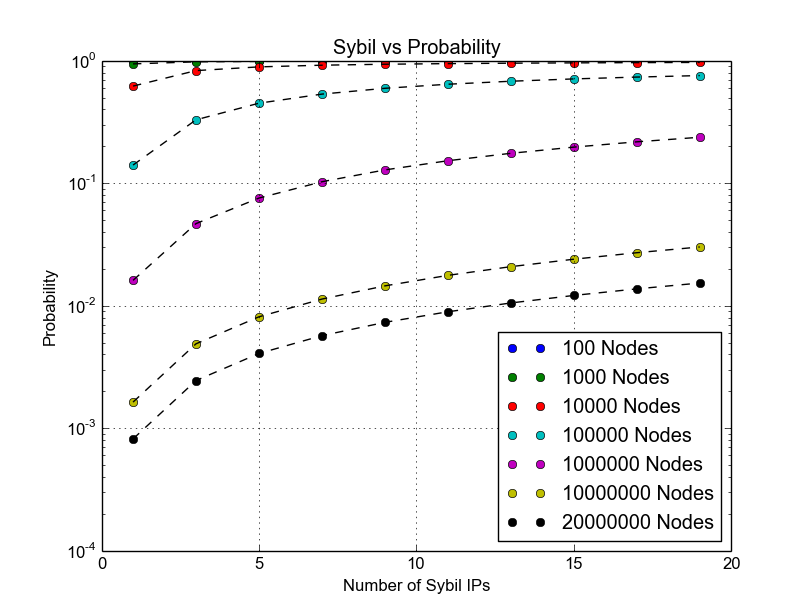
\includegraphics[width=0.65\linewidth]{ip_prob_all}
            \caption[foo]{Our simulation results.  
                The $x$-axis corresponds to the number of IP addresses the adversary can bring to bear.
                The $y$-axis is the probability that a random region between two adjacent normal members of the network can be mashed.
                Each line maps to a different network size of $n$.
                The dotted line traces the line corresponding to the Equation \ref{eq:bad}: $ P_{bad\_neighbor} =  \frac{num\_ips \cdot 16383}{num\_ips \cdot 16383 + n - 1}$}.
            \label{fig:exp2}
        \end{figure}
    \end{frame}
    
    \begin{frame}
        
        \begin{figure}
            \centering
            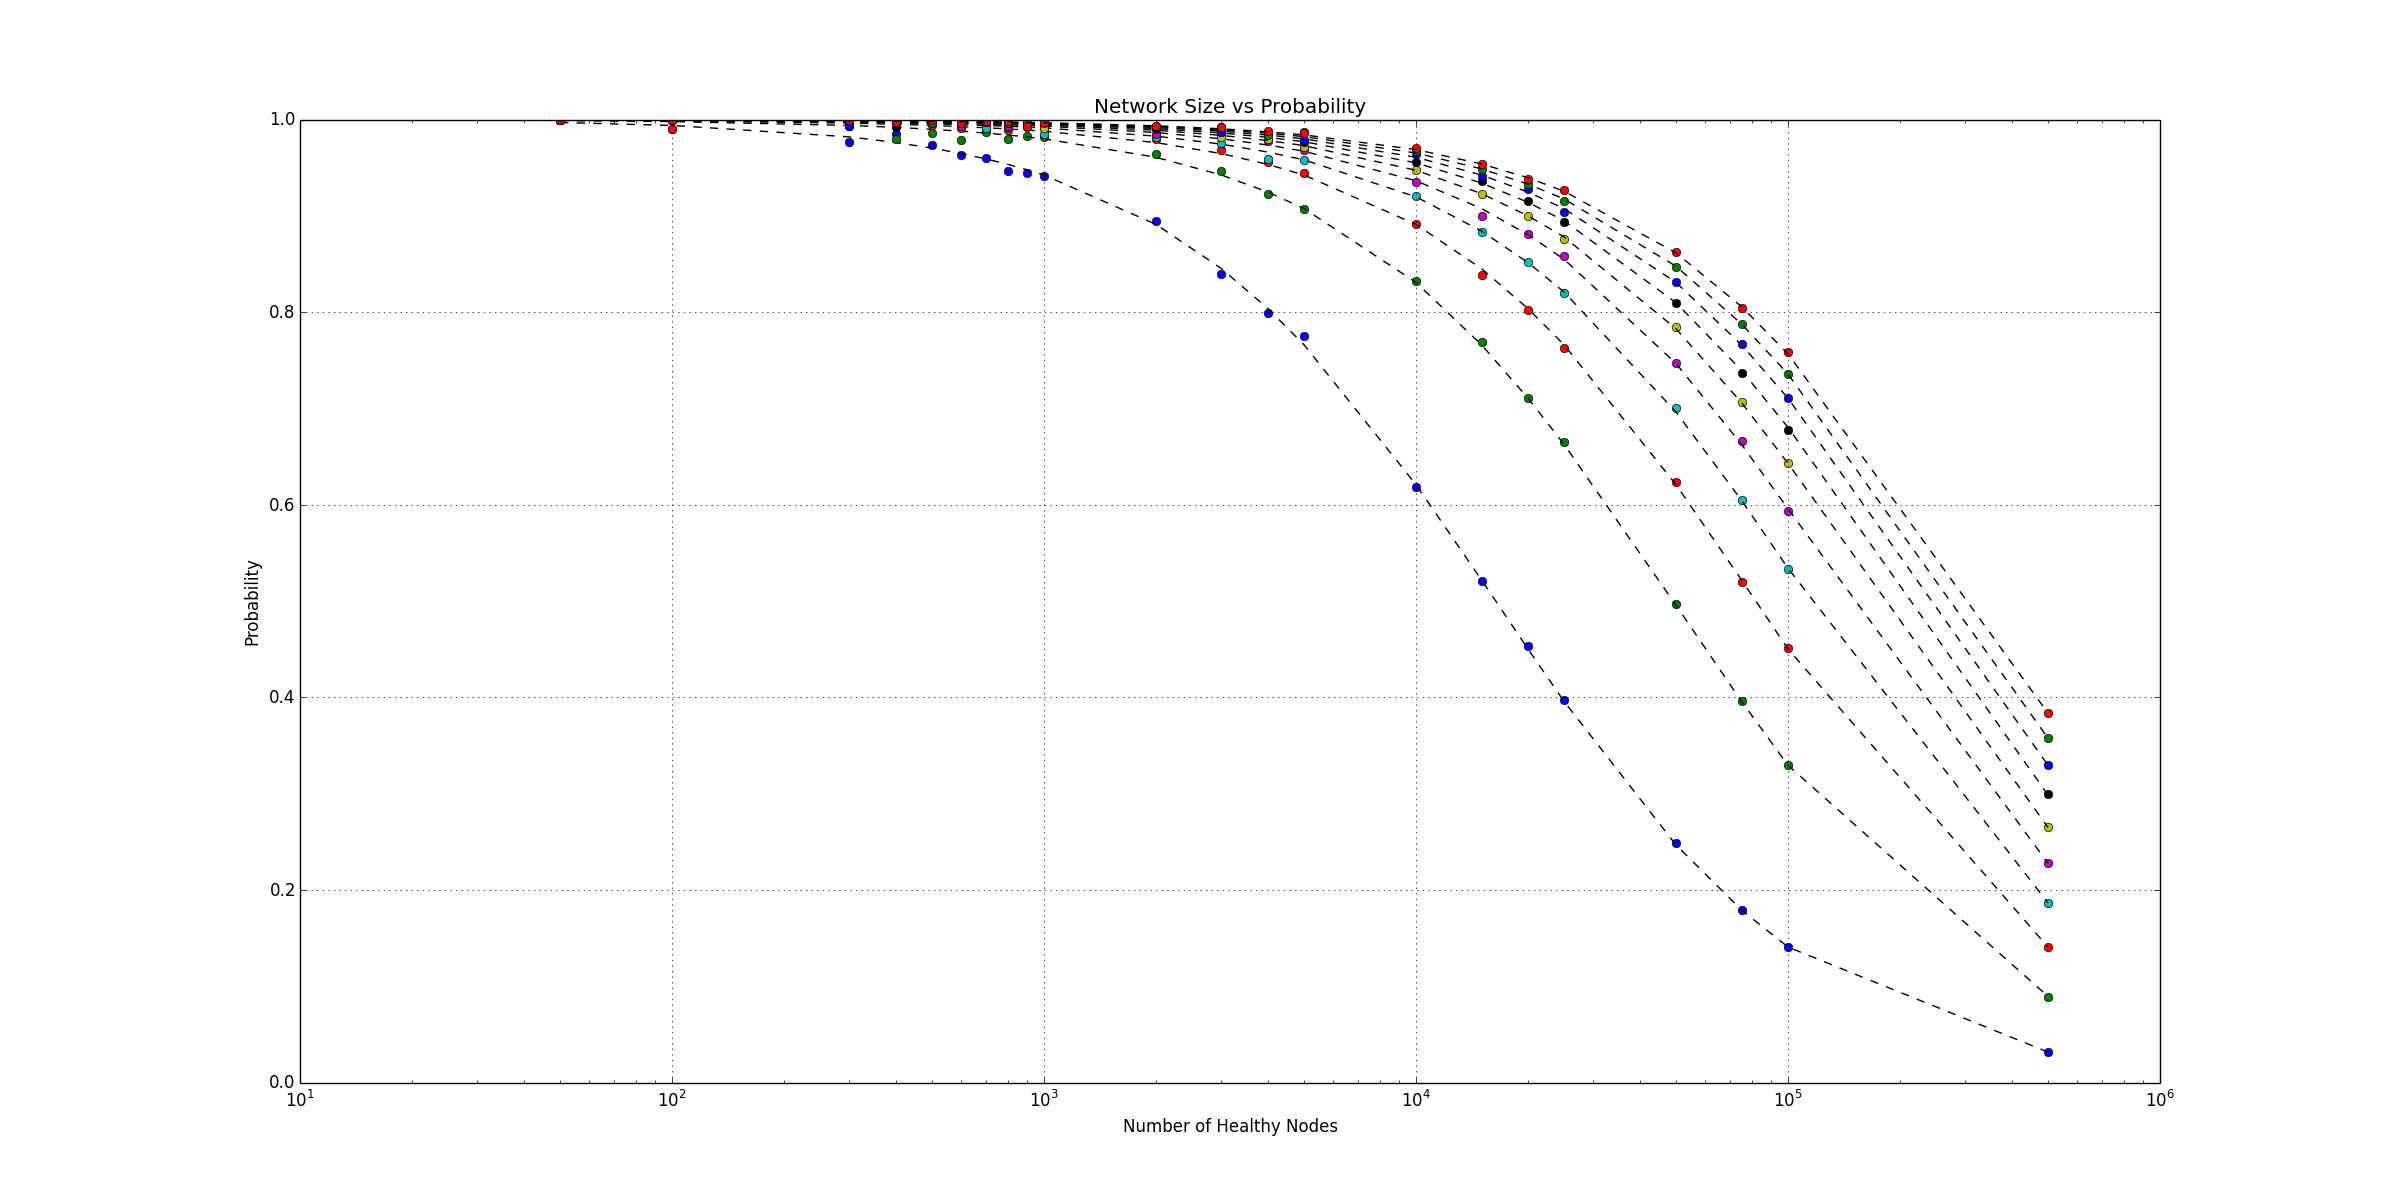
\includegraphics[width=0.7\linewidth]{size_prob_all}
            \caption[a]{These are the same as results shown in Figure \ref{fig:exp2}, but our $x$-axis is the network size $n$ in this case.  
                Here, each line corresponds to a different number of unique IP addresses the adversary has at their disposal.}
            \label{fig:size_prob_all}
        \end{figure}
    \end{frame}
    
    \begin{frame}
        \begin{figure}
            \centering
            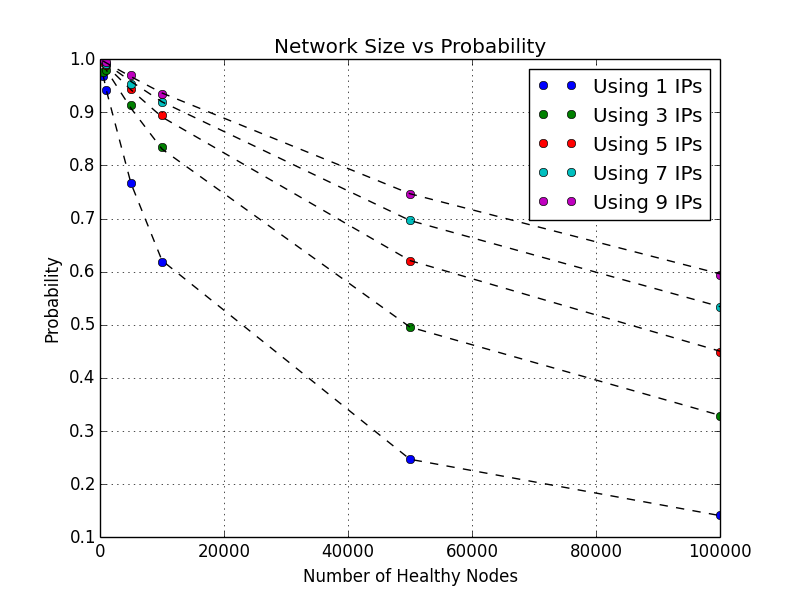
\includegraphics[width=0.7\linewidth]{size_occlusion_chord}
            \caption{This graph shows the relationship between the network size and the probability a particular link, adjacent or not, can be mashed.}
            \label{fig:exp3}
        \end{figure}
    \end{frame}
    
    
    \begin{frame}
        Questions?
    \end{frame}

    \bibliography{potato}
    \bibliographystyle{plain}
    
\end{document}